\chapter{Evaluation}\label{ch:eval}
\label{sec:eval:overall}

The project fulfilled all its success criteria and was successfully completed.

A large subset of Beam features were implemented (\cref{sec:eval:limitations}).
The programmer interface which was developed followed patterns native to Elixir.
It resulted in a low-impedance translation from a conceptual Dataflow Pipeline to its representation in code, achieving a dramatic reduction in code size over a Java version (\cref{sec:eval:twitter:code}).

The project implementation also displayed performance superior to the single-machine Beam runner, proving able to deal with busy streams of data and large Pipelines while displaying excellent latency characteristics and a predictable, linear performance response to load (\cref{sec:eval:latency}).
The Beam runner was not able to handle the stream of data even with very simple Pipelines.

The final project weighed in at approximately \num{3200} lines of Elixir code (excluding comments, blank lines and tests).
Approximately \num{12000} lines of code were written over the lifetime of the project, illustrating the volatility of the codebase due to evolving requirements.

In comparison, the core Beam codebase comprises $\sim$\num{78000} lines of code, though it implements some functionality which is out-of-scope for the Elixir implementation.

\section{Feature analysis}\label{sec:eval:limitations}

The Beam Capability Matrix~\cite{Beam-Cap-Matrix} is a standard method of feature comparison among Beam implementations.
\Cref{tab:eval:capability} shows the Capability Matrix augmented with a column indicating features implemented during this project.

\newcommand{\pmark}{$\sim$}
\begin{table}
	\caption[Apache Beam Capability Matrix including the Elixir implementation.]{The Capability Matrix~\cite{Beam-Cap-Matrix} compares support for Beam Model features across implementations. The~\pmark~symbol indicates a partial implementation.}
	\label{tab:eval:capability}	
	\tabulinesep=1.4mm
	\begin{tabu}{|X[2.8,r,m]|X[c,m]|X[c,m]|X[c,m]|X[c,m]|X[c,m]|} \firsthline
		& \textbf{Beam Model} & \textbf{Google Cloud Dataflow} & \textbf{Apache Flink} & \textbf{Apache Spark} & \textbf{Elixir} \\ \hline\hline
		
		\multicolumn6{|c|}{\textbf{What is being computed?}} \\ \hline
		%\tabuphantomline
		ParDo & \cmark & \cmark & \cmark & \cmark & \cmark \\ \hline
		GroupByKey & \cmark & \cmark & \cmark & \pmark & \cmark \\ \hline
		Flatten & \cmark & \cmark & \cmark & \cmark & \xmark \\ \hline
		Combine & \cmark & \cmark & \cmark & \cmark & \cmark \\ \hline
		Composite Transforms & \cmark & \pmark & \pmark & \pmark & \pmark \\ \hline
		Side Inputs & \cmark & \cmark & \cmark & \cmark & \xmark \\ \hline
		Source API & \cmark & \cmark & \cmark & \cmark & \xmark \\ \hline
		Aggregators & \pmark & \pmark & \pmark & \pmark & \xmark \\ \hline
		Stateful processing & \cmark & \pmark & \pmark & \xmark & \xmark \\ \hline\hline
		
		\multicolumn6{|c|}{\textbf{Where in event-time?}} \\ \hline
		Global windows & \cmark & \cmark & \cmark & \cmark & \cmark \\ \hline
		Fixed windows & \cmark & \cmark & \cmark & \cmark & \cmark \\ \hline
		Sliding windows & \cmark & \cmark & \cmark & \cmark & \cmark \\ \hline
		Session windows & \cmark & \cmark & \cmark & \cmark & \pmark \\ \hline
		Custom windows & \cmark & \cmark & \cmark & \cmark & \cmark \\ \hline
		Custom merging windows & \cmark & \cmark & \cmark & \cmark & \pmark \\ \hline
		Timestamp control & \cmark & \cmark & \cmark & \cmark & \cmark \\ \hline
		Watermark domains & \xmark & \xmark & \xmark & \xmark & \cmark \\ \hline \hline
		
		\multicolumn6{|c|}{\textbf{When in processing-time?}} \\ \hline
		Configurable triggering & \cmark & \cmark & \cmark & \xmark & \cmark \\ \hline
		Event-time triggers & \cmark & \cmark & \cmark & \xmark & \cmark \\ \hline
		Processing-time triggers & \cmark & \cmark & \cmark & \cmark & \xmark \\ \hline
		Count triggers & \cmark & \cmark & \cmark & \xmark & \pmark \\ \hline
		(Meta)data-driven triggers & \xmark & \xmark & \xmark & \xmark & \xmark \\ \hline
		Composite triggers & \cmark & \cmark & \cmark & \xmark & \pmark \\ \hline
		Allowed lateness & \cmark & \cmark & \cmark & \xmark & \cmark \\ \hline
		Timers & \cmark & \pmark & \pmark & \xmark & \pmark \\ \hline \hline
		
		\multicolumn6{|c|}{\textbf{How do refinements relate?}} \\ \hline
		Discarding mode & \cmark & \cmark & \cmark & \cmark & \cmark \\ \hline
		Accumulating mode & \cmark & \cmark & \cmark & \xmark & \cmark \\ \hline
		Retractions & \xmark & \xmark & \xmark & \xmark & \xmark \\ \lasthline
	\end{tabu}
\end{table}

As the Matrix demonstrates, no implementation is feature-complete in spite of Beam containing core Java classes to be used as the basis for each feature implementation---something this project could not take advantage of.
Over the course of this Part~II project, a significant subset of features were implemented.
The only limitation not shown in \cref{tab:eval:capability} is the lack of support for non-linear Pipelines.

Some core modules were implemented using na\"ive algorithms to save on time.
For instance, a linear list-based priority queue was used in the core of several grouping and windowing algorithms.
In spite of this, the performance of the implementation was excellent, as the rest of this chapter shows.

\section{Approach to empirical evaluation}\label{sec:eval:approach}

\subsection{Test environment}\label{sec:eval:approach:environment}

Efforts were made to collect data in similar environments in order to reduce the potential for uncontrolled variation.

All tests were conducted on a MacBook Pro (15-inch, Late 2016) with a \SI{2.9}{\giga\hertz} Intel Core~i7 CPU and \SI{16}{GB} of \SI{2133}{\mega\hertz} RAM running macOS 10.12.4.
Runtimes used were Elixir 1.4.2 on OTP 19 and the Oracle JRE v1.8.0\_66-b17.

Prior to conducting the tests, all non-essential background processes and applications were terminated.
Tests were initiated using a scripted test runner in order to replicate multiple instances of the tests accurately.

\subsection{Data collection and processing methodologies}\label{sec:eval:approach:collection}

A custom test runner was developed in Elixir for the purpose of scheduling and running tests.
It could be configured with tests for both the Java and Elixir implementations.
Each test was executed via a new system process with configuration passed as command-line arguments.
A new VM instance was spawned each time for both Elixir and Java tests to maintain consistency and accuracy.

The test runner measured the CPU and memory usage of the spawned process using the \verb|ps| program.
Other measurements, such as latency, were recorded directly by the instrumented binary.

The data were then processed, analysed and plotted using MATLAB.
Sources for both the test runner and the MATLAB scripts used can be found in \cref{apx:twitter-code}.

\section{The Twitter example}\label{sec:eval:approach:twitter}

Twitter is a popular social network focused on posting short messages, or \emph{statuses}.
Statuses tend to include \emph{hashtags}, words or short phrases preceded by the \# character.
Hashtags rely on many users using the exact hashtag text in their tweets.
The hashtag can then be used to aggregate and list all of these tweets, perhaps on a particular topic.

An autocomplete functionality would be useful when composing tweets to suggest popular hashtags and discourage misspellings.
This real-world scenario formed the basis of this evaluation exercise.

Twitter's free streaming API~\cite{TwitterStreamingAPI} was used to receive a stream of English-language tweets on particular topics.
Thirteen terms pertaining to technology (such as `tech' and `Google') were selected and passed to the API to constrain the results.

\todo{rework below}

The tweets were windowed using sliding windows and then processed further.
Hashtags present were counted per-window.
They were then expanded into all possible prefixes, retaining counts.
Finally, a list of the top three hashtag suggestions for each prefix was produced.
This data could be fed into an autocompletion API, but for the purposes of this exercise was simply logged.
\Cref{fig:eval:twitter-pipeline-dag} illustrates the resultant Pipeline.

\begin{figure}
	\centering
	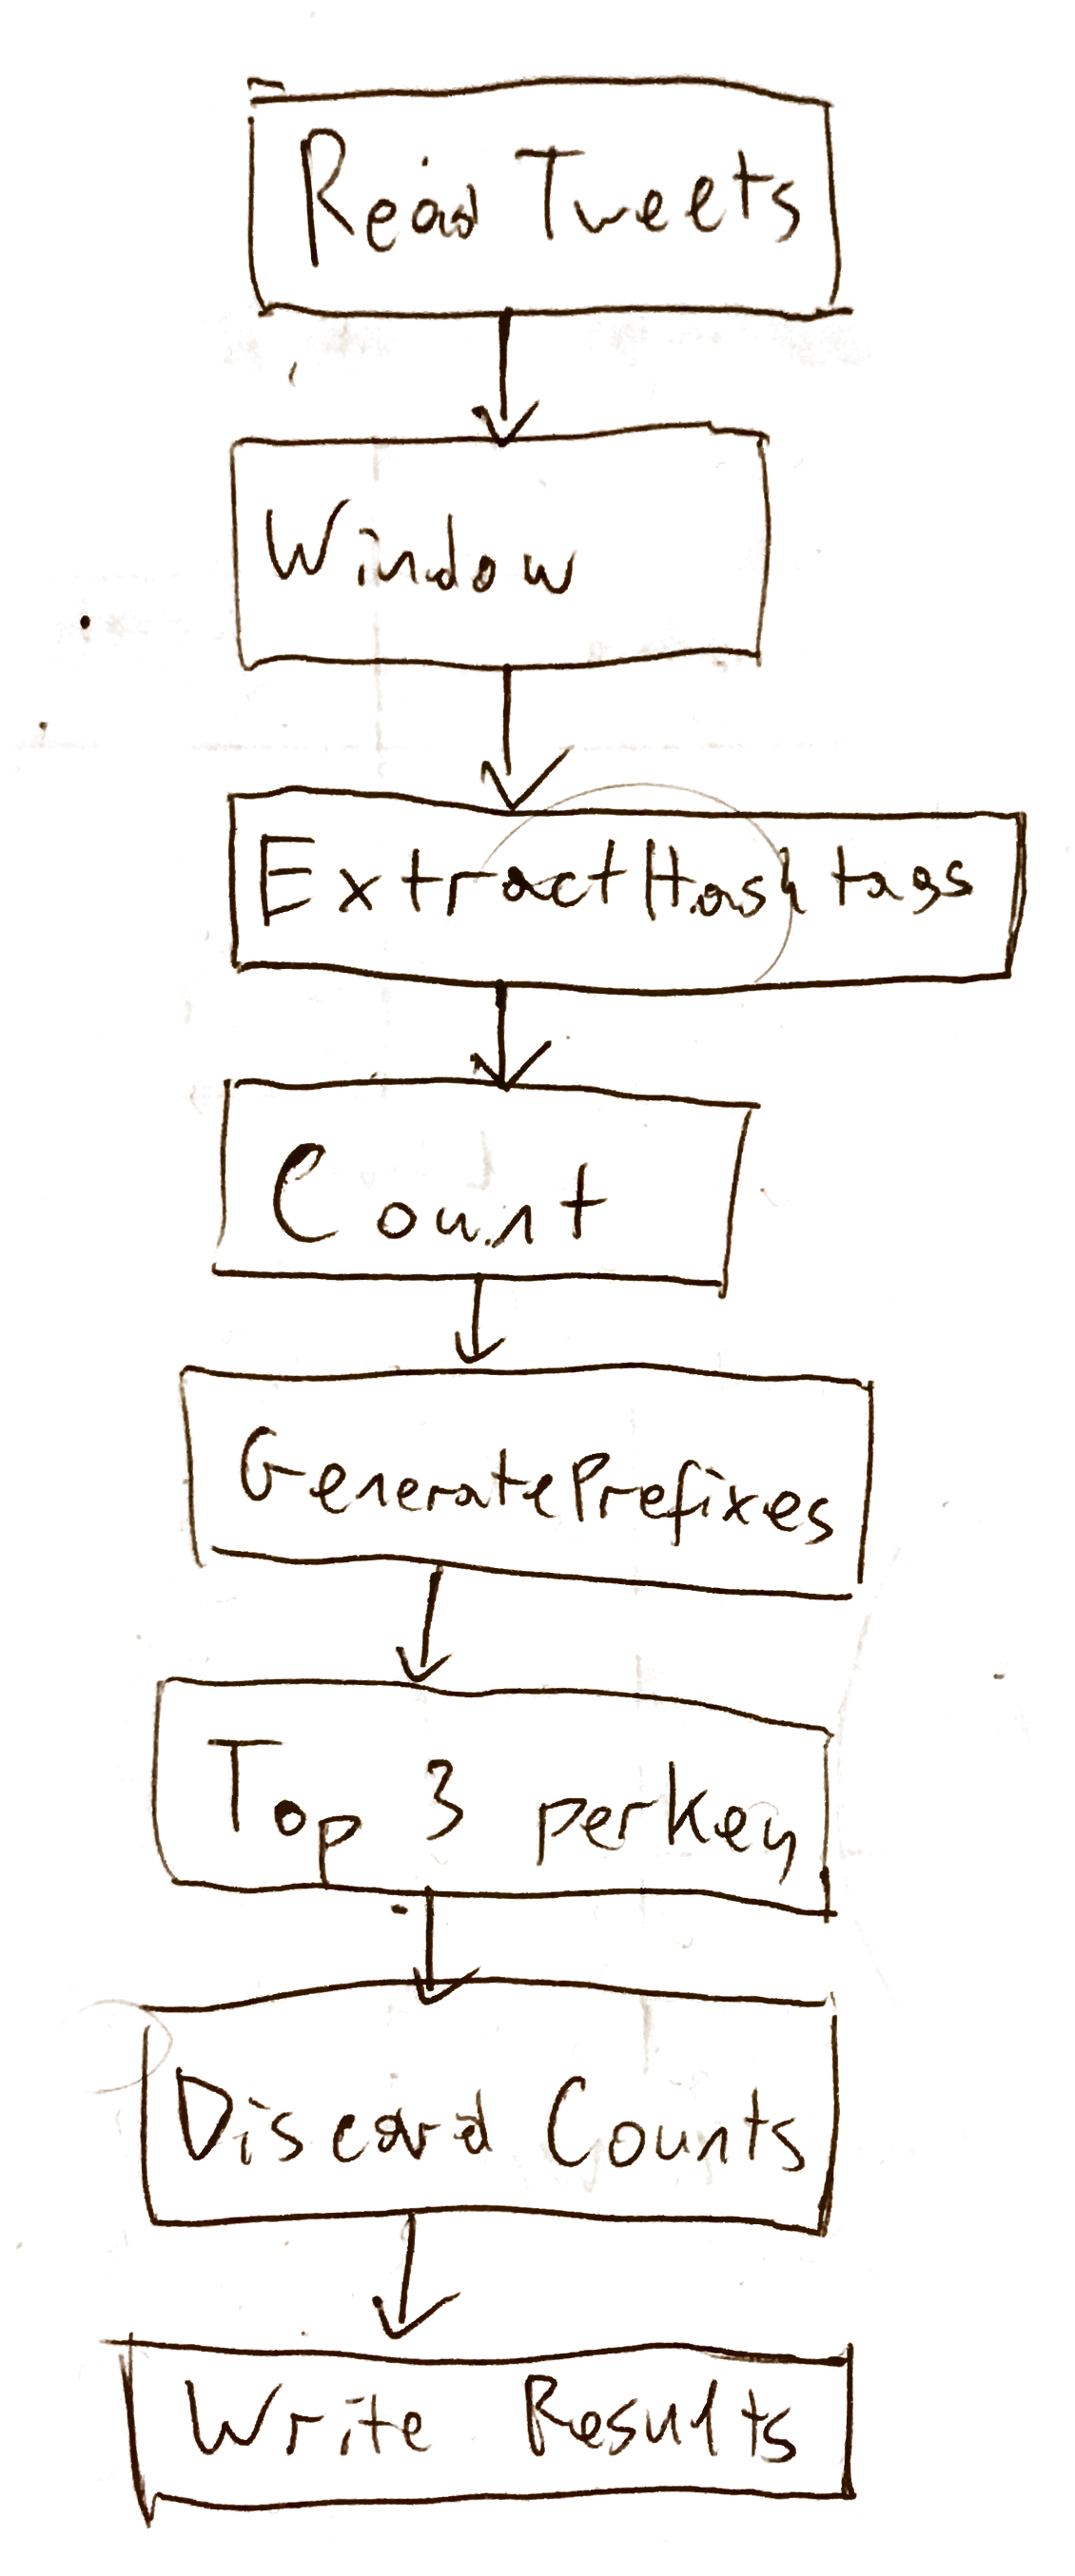
\includegraphics[height=0.5\textheight]{images/temp/eval-twitter-pipeline}
	\caption[The Twitter example Pipeline as a Directed Acyclic Graph.]{The Twitter example uses a Pipeline representative of a real-world application. The lines-of-code needed to implement each step in the Pipeline are also shown.}
	\label{fig:eval:twitter-pipeline-dag}
\end{figure}


The scenario provides a good way to test various features of the Model.
Sliding windowing is used, and multiple stages of aggregation per window is employed.
The Pipeline utilises both Elementwise and Grouping Transforms.

The free stream provided by Twitter delivers only around 50--80 tweets/second.
Therefore, to exercise the systems and compare their performance under load, both Pipelines included a configurable step which duplicated the tweets by a multiplicative factor, simulating a higher-volume stream.

The key success criterion in this example is not necessarily throughput or latency, due to the bounded amount of input and output per window.
Rather, success is defined as the ability to deliver results on time for each window.

\subsection{Code comparison}\label{sec:eval:twitter:code}

The Pipeline was created in both the Java and Elixir implementations of the Model.
The full code is available in \cref{apx:twitter-code}; what follows is a comparison of selected excerpts which illustrate the differences in the two coding styles.

The Java example is noticeably longer, using XX lines of code (excluding blank lines and comments).
In contrast, the Elixir implementation takes only XX lines of code to write.

\subsubsection{Reading tweets}

One of the primary reasons for the length of the Java version is the required method of injecting the stream of tweets into the Pipeline.

\begin{codelisting}
	\caption{Reading a Twitter stream as an unbounded source in Elixir.}
	\label{lst:eval:twitter-readstream-elixir}
	\begin{minted}[breaklines=true]{elixir}
parse_as_timestamp = fn string ->
  string
  |> Timex.parse!("{WDshort} {Mshort} {0D} {h24}:{0m}:{0s} {Z} {YYYY}")
  |> DateTime.to_unix
  |> DTime.timestamp(:seconds)
end
terms = [...]
#...
p
~> "Read Stream" -- IO.read_stream(fn -> ExTwitter.stream_filter(track: terms, language: "en") end)
~> "Extract Timestamps" -- Windowing.with_timestamps(&parse_as_timestamp.(&1.created_at),
     delay_watermark: {30, :seconds, :event_time})
# `&parse_as_timestamp.(&1.created_at)` is captured lambda syntax for
# fn tweet -> parse_as_timestamp.(tweet.created_at) end
	\end{minted}
\end{codelisting}

\begin{codelisting}
	\caption[Reading a Twitter stream as an unbounded source in Java.]{Reading a Twitter stream as an unbounded source in Java. Code compressed for readability, the full version (\cref{lst:apxb:twitter-java}) is 194 LoC.}
	\label{lst:eval:twitter-readstream-java}
	\begin{minted}[breaklines=true]{java}
static class DummyCheckpoint
    implements UnboundedSource.CheckpointMark, Serializable { /*...*/ }
    
static class TwitterSource
    extends UnboundedSource<Status, DummyCheckpoint> {
    /*...*/
        
    @Override
    public UnboundedReader<Status> createReader(
        PipelineOptions options,
        @Nullable DummyCheckpoint checkpointMark
    ) throws IOException { /*...*/ }

    protected static class Reader
    extends UnboundedSource.UnboundedReader<Status>
    implements StatusListener {
        /*...*/
        private Reader(String[] terms, TwitterSource source) { /*...*/ }
        @Override public boolean start() throws IOException { /*...*/ }
        @Override public boolean advance() throws IOException { /*...*/ }
        @Override public Status getCurrent() throws NoSuchElementException { /*...*/ }
        @Override public Instant getCurrentTimestamp() throws NoSuchElementException { /*...*/ }
        @Override public void close() throws IOException { /*...*/ }
        @Override public Instant getWatermark() { /*...*/ }
        /*...*/
        @Override public void onStatus(Status status) { /*...*/ }
        /*...*/
    }
}
/*...*/
String[] terms = {/*...*/};

p.apply("GetTweets", Read.from(TwitterSource.withTerms(terms)))
	\end{minted}
\end{codelisting}

The Elixir standard library provides a way to deal with potentially unbounded, lazy data---\exs{Stream}s.
As such, it makes sense that one of the Root Transforms provided out of the box in Elixir Dataflow is \exs{IO.read_stream}.
We need only pass a lambda which creates the desired stream on-demand, and its elements will automatically be emitted.

\Cref{lst:eval:twitter-readstream-elixir} illustrates this well.
\exs{ExTwitter} is a Twiter client for Elixir, and indeed it uses the standard \exs{Stream} module to provide its functionality.

Notable is the ease with which we can timestamp elements based on their data, and assign them a watermark with a simple, standard Transform.
\exs{Windowing.with_timestamps} is a Composite Transform, so it is easy to insert a smarter watermark heuristic if needed; the one used takes the highest timestamp seen so far and outputs a watermark 30 seconds before this---an element can be up to 30 seconds `out of order' before it is considered late.
This showcases the watermark domains feature (\cref{sec:impl:dataflow:watermark-generation}) not present in the Java implementation.
It is possible to decouple the reading of the stream and the timestamp extraction and watermark generation into separate Transforms, resulting in cleaner, more reusable code.

To achieve the same result in Java (\cref{lst:eval:twitter-readstream-java}), almost 200 lines of code are needed.
Firstly, since there is no standard way of representing streaming sequences in Java, custom sources of data will need to implement their own asynchronous logic.
\texttt{Twitter4J}, a popular Twitter client library for Java, requires the user to provide a callback object implementing a particular interface to be notified of new tweets.

In order to `connect' the Twitter stream to the Pipeline, an \texttt{UnboundedSource} had to be written.
This is a large interface requiring the implementation of several functions.
Some of these apply to the advanced distributed features offered by Beam such as checkpointing and coding\footnote{
Used to dump data from memory into storage. In Elixir, no extra coding logic is needed since any term can be serialised in a standard way.
} and are omitted.
Others, however, show the incidental complexity present in the Java API.
On top of this, care must be taken to ensure the class is thread-safe.

Since Beam assumes that the entire Pipeline is in the same watermark domain, the Source itself must manage its own timestamping and watermark generation.
In this case, the class must contain logic not only to read, buffer and emit tweets from the network, but also to extract their timestamp and to generate the delayed watermark based on the data.
This results in long, tightly-coupled and complex code.

Clearly, the conventions around \exs{Stream}s in Elixir coupled with the decoupling of reading and processing logic due to the inclusion of watermark domains combine to demonstrate that the Elixir solution is superior.

\subsubsection{Lambdas vs.\ classes}

The Dataflow Model adopts an inherently functional model of computation based on functions transforming data, often using standard patterns of mapping and filtering.
Java's support for this model is poor.
This is exemplified best by the common need to specify logic in small internal classes as in \cref{lst:eval:twitter-lambdas-java}.

\begin{codelisting}
	\caption[Using internal classes to specify transformation logic in Java.]{In Java, there is often a need to use internal classes to specify logic. While Java~8 lambdas can be used, the lack of  type inference means that internal classes are often a cleaner solution.}
	\label{lst:eval:twitter-lambdas-java}
	\begin{minted}[breaklines=true]{java}
 public static class GeneratePrefixesFn
 extends SimpleFunction<KV<String, Long>, List<KV<String, KV<String, Long>>>> {
    @Override
    public List<KV<String, KV<String, Long>>> apply(KV<String, Long> tagWithCount) {
        List<KV<String, KV<String, Long>>> result = new ArrayList<>();
        String downcased = tagWithCount.getKey().toLowerCase();
        for (int i = 1; i <= downcased.length(); i++) {
            String prefix = downcased.substring(0, i);
            result.add(KV.of(prefix, tagWithCount));
        }
     return result;
    }
}
public static class DiscardCountsFn
extends SimpleFunction<KV<String, List<KV<String, Long>>>, KV<String, List<String>>> {
    @Override
    public KV<String, List<String>> apply(KV<String, List<KV<String, Long>>> el) {
        List<String> prefixes = l.getValue().stream().map((KV::getKey)).collect(Collectors.toList());
        return KV.of(el.getKey(), prefixes);
    }
}
/*...*/
.apply("GeneratePrefixes", FlatMapElements.via(new GeneratePrefixesFn()))
/*...*/
.apply("DiscardCounts", MapElements.via(new DiscardCountsFn()))
	\end{minted}
\end{codelisting}

\begin{codelisting}
	\caption[Using lambdas to specify transformation logic in Elixir.]{In Elixir, we take advantage of the inherent functional paradigm of the language to specify transformation logic in a familiar way.}
	\label{lst:eval:twitter-lambdas-elixir}
	\begin{minted}[breaklines=true]{elixir}
~> "Generate Prefixes" -- Core.flat_map(fn {tag, count} ->
  len = String.length tag
  for i <- 0..(len-1), downcased = String.downcase(tag),
    prefix = String.slice(downcased, 0..i),
    do: {prefix, {tag, count}}
 end)
# ...
~> "Discard Exact Counts" -- Core.map(fn {prefix, tcs} ->
  {prefix, Enum.map(tcs, fn {tag, _count} -> tag end)}
 end)
	\end{minted}
\end{codelisting}

\Cref{lst:eval:twitter-lambdas-elixir} shows that Elixir, as a functional language, excels at expressing these kinds of computation natively.

\subsubsection{Summary}

Though formal user studies were not performed to assess the `friendliness' or ease of use of the two SDKs empirically, the preceding examples show that Elixir as a language is much better suited to express the concepts of the Dataflow Model in code.
Java's paradigm is orthogonal to the way computation is reasoned about in the Model, and even though a `fluent API' can be used to make things as friendly as possible, the static typing coupled with no type inference fundamentally limits the expressivity of the language in uses like this one.


\subsection{Performance evaluation}\label{sec:eval:performance}

\subsection{Resource consumption}\label{sec:eval:resource}

\section{Latency evaluation}\label{sec:eval:latency}

A key performance indicator of stream-processing systems is the latency of a single element from input to output when the system is under load.
Notwithstanding the Model's powerful windowing features, implementations must display robust streaming performance if they are to subsume existing systems.

\subsection{Methodology}

In this experiment, a Pipeline was created in which integer elements were generated uniformly at a rate of \SI{100}{\per\second} and passed through a series of \verb|Map| Transforms, each of which incremented the value.
The latency of each element was measured from the moment of its generation to its output at the last Transform.
The length of the Pipeline was varied and the effects on element latency analysed.
CPU and memory usage were also captured at half-second increments.

The experiment compared the performance of the Elixir implementation with the Apache Flink runner, an optimised, production-ready runner for Beam.
The Beam DirectRunner, the default for local Pipelines, was also tested but could not achieve the throughput necessary for its data to be comparable.

Streaming Pipelines tend to be long-running. As such, the first \SI{10}{\second} of data was discarded, as the Java runners showed a large spike in resource usage and element latency while the Pipeline was initialising.
The Elixir runner displayed a similar spike, which was usually shorter than \SI{1}{\second}.

Each instance of the experiment was repeated \num8 times, each time running for \SI{180}{\second}.

\subsection{Runner choice}

The initial experimental design evaluated Pipeline lengths of up to \num{10000} Transforms, comparing the project implementation to the Beam DirectRunner.
However, the DirectRunner ran out of stack space when trying to construct Pipelines longer than $\sim$\num{2000} Transforms.
Given that such large Pipelines are uncommon in practice, the length range was modified to \num{10}--\num{2000} Transforms.

After analysis of the data was carried out, it emerged that the DirectRunner could not in fact handle a \SI{100}{\per\second} stream of elements---the limiting factor was throughput, not latency.
\Cref{fig:eval:latency-graph-java} illustrates the situation.
The element latency consistently grew with time as the test ran.
This indicates that the runner was falling behind the stream and could not process it in real-time.
This occurred with CPU usage consistently close to \SI{100}{\percent} (even though \num8 hyperthreads were available) and memory usage at \pmark\SI{1.2}{GiB} (even though the heap size was \SI{4}{GB}).
This indicated that the bottleneck was due to the single-threaded design of the runner.
Indeed, it could not even handle a full stream of elements at a rate of \SI{10}{\per\second}.

In order to obtain data suitable for a meaningful comparison, the experiment was re-run using the Apache Flink \cite{ApacheFlinkRunner} runner.
The Apache Flink project has focused on implementing the Beam Model and is the production-ready open-source runner most suitable and optimised for execution of Beam Pipelines \cite{ApacheFlinkFocus}.
While it supports cluster execution, it was run locally to obtain comparable data.
However, even with the stack size increased to \SI{256}{MB}, it could not construct Pipelines longer than \pmark\num{500} Transforms, and so the range of Pipeline lengths evaluated was reduced.

\begin{figure}
    \centering
	\subfloat[][\textbf{DirectRunner: Element latencies with time at different Pipeline lengths}\\ $N$ is the number of Transforms. Multiple executions are shown per plot. The rate of latency growth increases with the Pipeline length.]{
		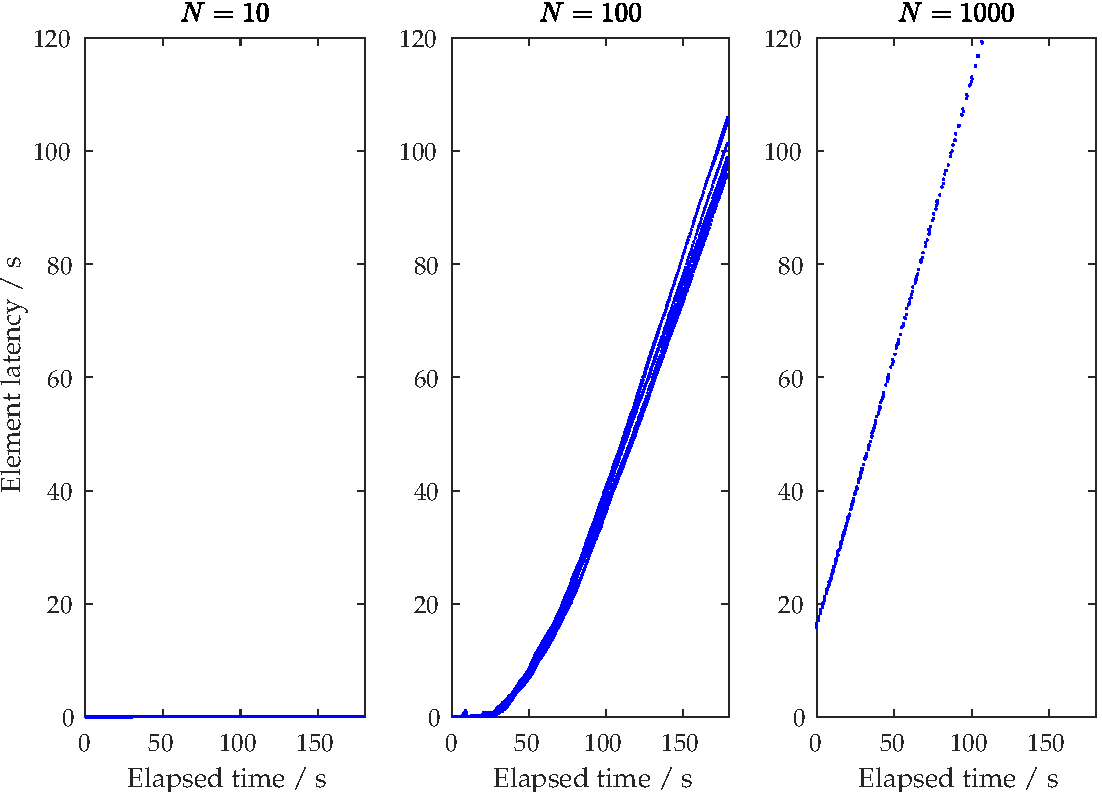
\includegraphics[height=0.42\textheight]{images/graphs/java_latency_demo}
	}
	
	\subfloat[][\textbf{DirectRunner: CPU and memory usage at different Pipeline lengths}\\The CPU and memory usage remained stable at lengths above \num{100} Transforms. The system did not consume all available resources (\SI{800}{\percent} CPU and \SI{4}{GB} memory).]{
		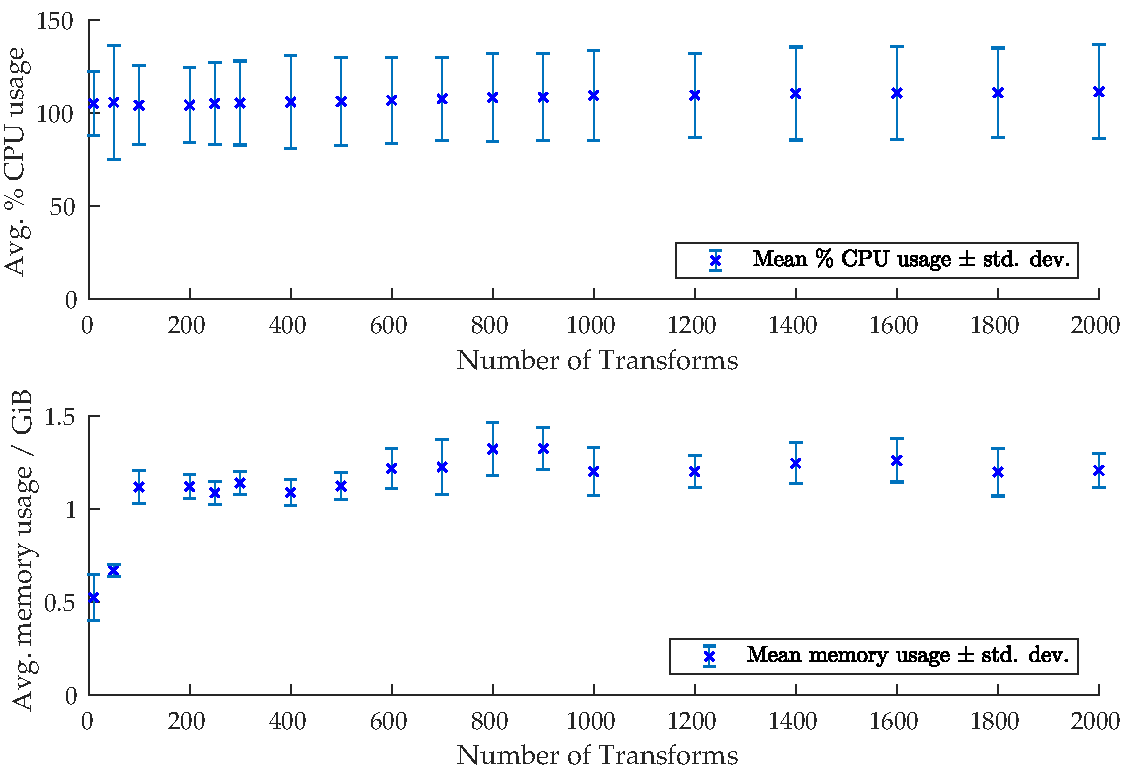
\includegraphics[height=0.42\textheight]{images/graphs/java_memcpu_double}
	}
	\caption[Results of the latency experiment executed on the DirectRunner, showing its unsuitability.]{The DirectRunner could not maintain sufficient throughput to evaluate the latency of the system under load in a valid way. Data indicate that this is due to the single-threaded design of the runner, not optimised for performance.}
	\label{fig:eval:latency-graph-java}
\end{figure}

\subsection{Results}

\subsubsection{Latency}

The Elixir runner displayed excellent performance, processing nearly all elements in less than \SI{10}{\milli\second} with a median of \SI8{\milli\second}, even at \num{2000} Transforms (\cref{fig:eval:latency-graph-elixir}\subref{fig:eval:latency-graph-elixir:latency}).

Both median latency and the inter-quartile range (IQR) increased with Pipeline length, indicating that in longer Pipelines elements experienced increased jitter.
This behaviour is likely due to the randomised scheduling of Transform processes by the BEAM.
The median latency and IQR both remained very low (cf. Flink) throughout the range of Pipeline lengths tested, suggesting excellent scalability across that dimension.

The Flink runner exhibited consistent---if unimpressive---latency results across the experimental range (which was smaller than that for Elixir) (\cref{fig:eval:latency-graph-flink}\subref{fig:eval:latency-graph-flink:latency}).
At all Pipeline lengths, the median latency was \SI{27}{\milli\second} with an IQR of \SI{13}{\milli\second}.
This shows that the runner is able to handle the element stream in this Pipeline length range, but points to another limiting factor.

\subsubsection{Resource consumption}

The Elixir runner displayed CPU usage and memory consumption which scaled linearly with Pipeline length, up to \SI{80}{\percent} and \SI{120}{MiB} at \num{2000} Transforms (\cref{fig:eval:latency-graph-elixir}\subref{fig:eval:latency-graph-elixir:cpumem}).
There is no indication that either of these resources were a limiting factor.
Instead, it is likely that the runner is prevented from achieving lower latencies by the overhead of switching and I/O between individual processes (Transforms).

The Flink runner also showed a linear trend in its resource consumption (\cref{fig:eval:latency-graph-flink}\subref{fig:eval:latency-graph-flink:cpumem}).
While its CPU usage was lower in the range tested (by a factor of \num{4}--\num{10}$\times$), its memory usage was significantly higher (by up to \num{60}$\times$) and growing fast with Pipeline length.
This pattern, when viewed against the consistent latency response in \cref{fig:eval:latency-graph-flink}\subref{fig:eval:latency-graph-flink:latency}, paints a picture of a system limited by memory operations.
The CPU usage is low because progress is often held back by memory operations.
This scenario is common in JVM applications.

\subsubsection{Conclusions}

The Elixir runner outperforms Flink with respect to latency across the experimental range, displaying \num{10}--\num{300}$\times$~lower median latency with significantly lower IQR.
It is able to maintain its excellent scalability at Pipeline lengths at which the Flink runner fails to initialise, in spite of not being designed with performance in mind.
This illustrates the power of the BEAM VM to execute extremely concurrent systems in a performant manner while maintaining low resource overheads.

The resource consumption of both runners scales linearly with Pipeline length, though Flink consumes as much as \num{60}$\times$~more memory in spite of lower CPU usage.
In practice, this pattern of memory consumption proves to be a limiting factor much before the CPU usage of Elixir does.

\begin{figure}
    \centering
	\subfloat[Element latency vs.\ Pipeline length.][\textbf{Elixir: Element latency vs.\ Pipeline length} \\An average of \num{128000} elements per box were measured. Each box shows the median and interquartile range. The outlier threshold is $1.5\times$ the IQR. Extreme outliers above \SI{12}{\milli\second} are omitted.]{
		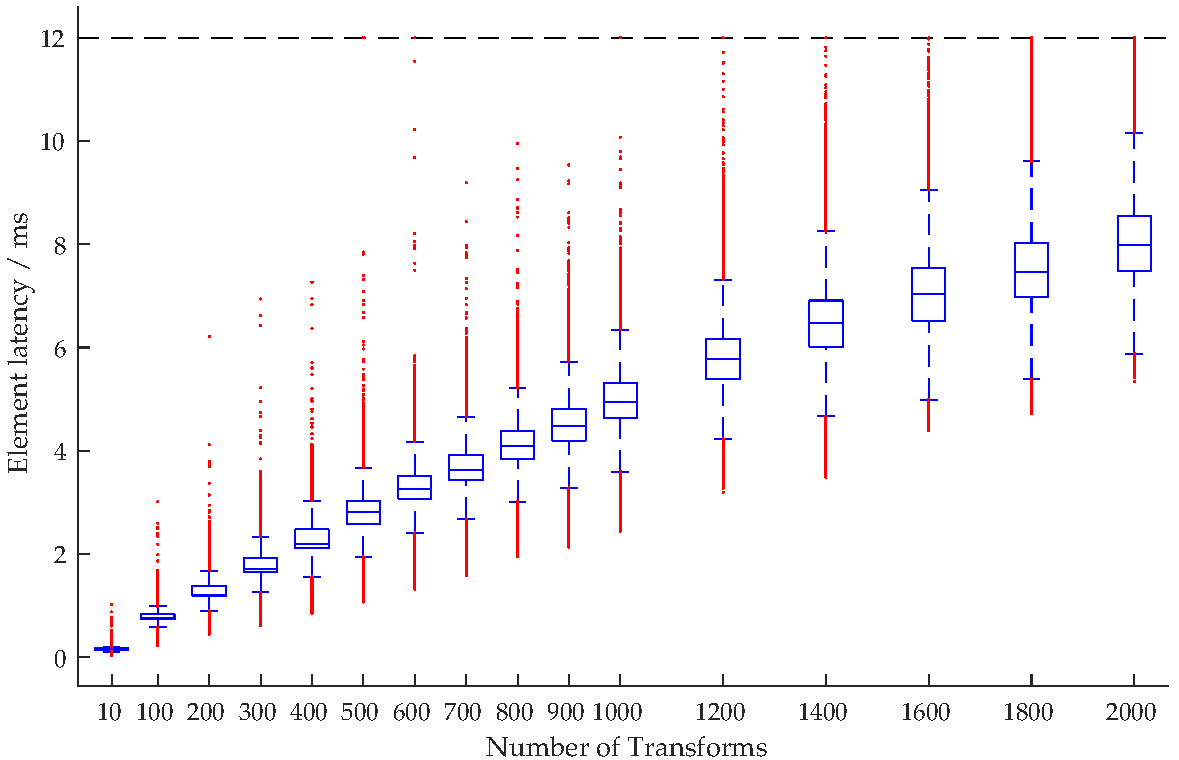
\includegraphics[height=0.42\textheight]{images/graphs/elixir_latency_box}
		\label{fig:eval:latency-graph-elixir:latency}
	}
	
	\subfloat[Average CPU and memory consumption vs.\ Pipeline length.][\textbf{Elixir: Average CPU and memory consumption vs.\ Pipeline length.} \\ Both resources are consumed with linear growth as the Pipeline length increases, as demonstrated by the good fit of a linear model.]{
		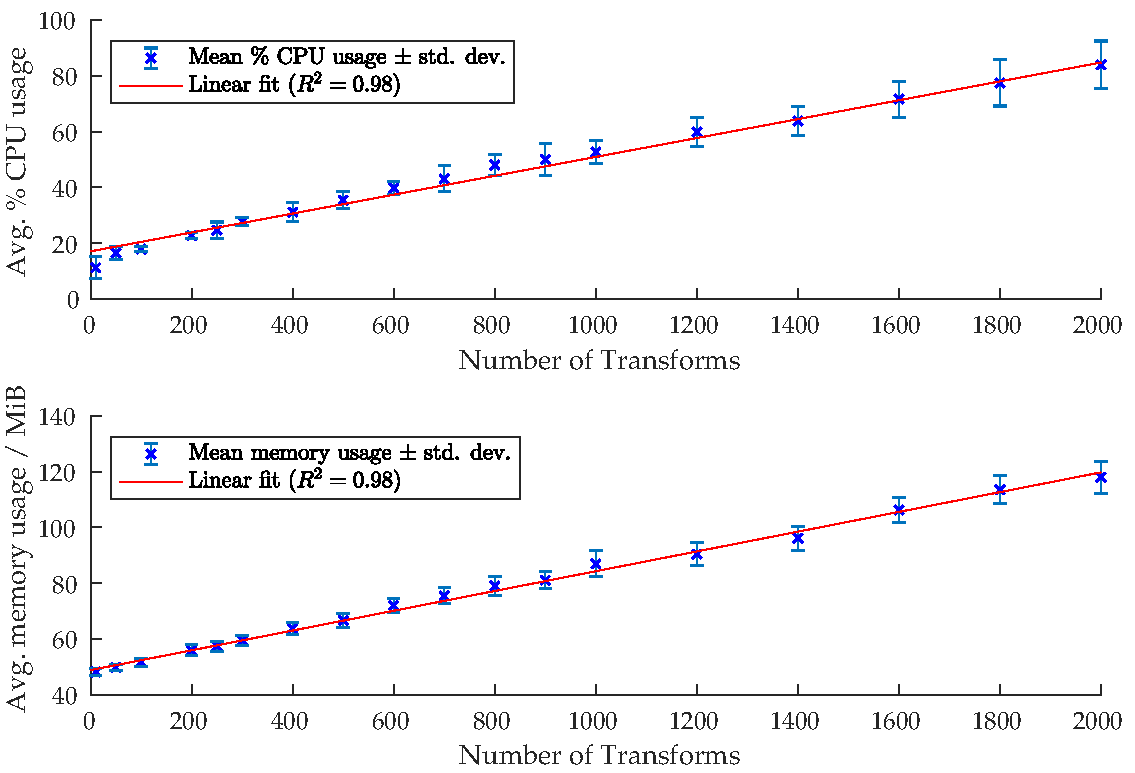
\includegraphics[height=0.42\textheight]{images/graphs/elixir_memcpu_linear}
		\label{fig:eval:latency-graph-elixir:cpumem}
	}
	\caption[Results of the latency experiment run executed on the Elixir runner.]{The Elixir runner exhibits good scalability under load. When processing elements at a rate of \SI{100}{\per\second}, even very long Pipelines maintain low latency and jitter while maintaining full throughput. Resource consumption scales linearly and predictably with Pipeline length.}
	\label{fig:eval:latency-graph-elixir}
\end{figure}

\begin{figure}
    \centering
	\subfloat[][\textbf{Flink: Element latency vs.\ Pipeline length} \\An average of \num{138000} elements per box were measured. Each box shows the median and interquartile range. The outlier threshold is $1.5\times$ the IQR. Extreme outliers above \SI{80}{\milli\second} are omitted.]{
		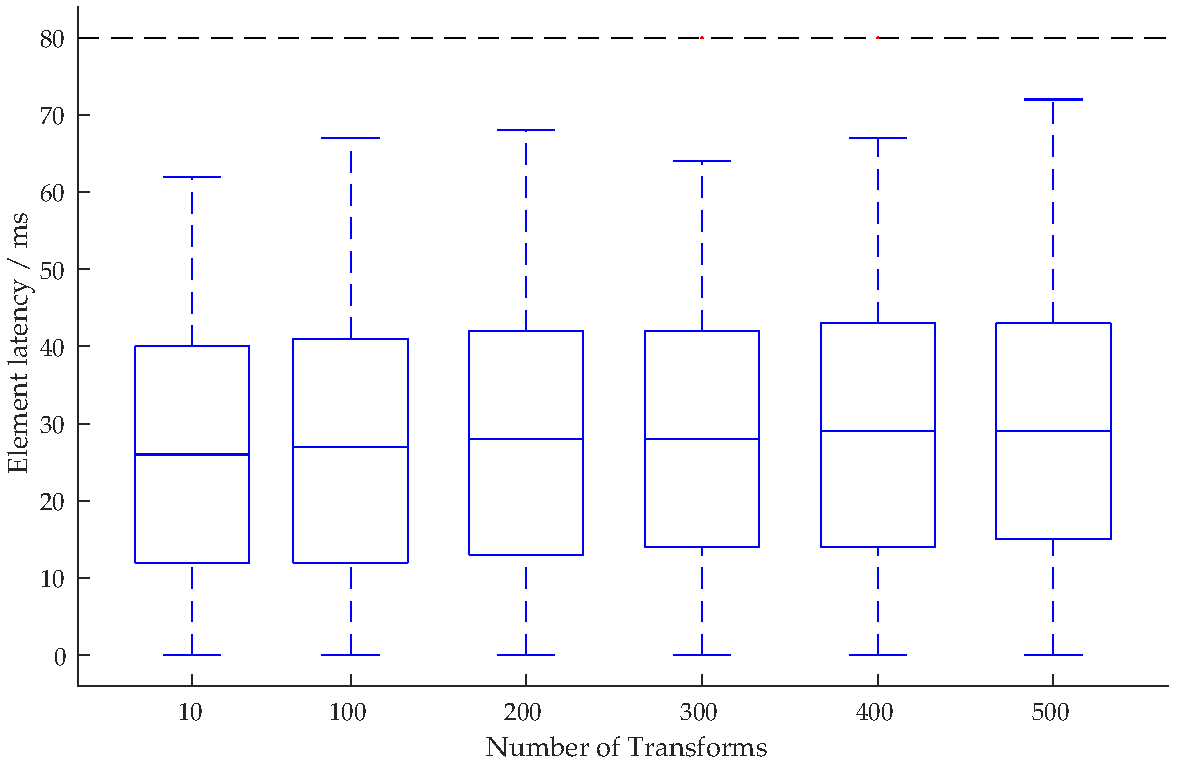
\includegraphics[height=0.42\textheight]{images/graphs/java_flink_latency_box}
		\label{fig:eval:latency-graph-flink:latency}
	}
	
	\subfloat[][\textbf{Flink: Average CPU and memory consumption vs.\ Pipeline length.} \\ Both resources are consumed with linear growth as the Pipeline length increases, as demonstrated by the good fit of a linear model.]{
		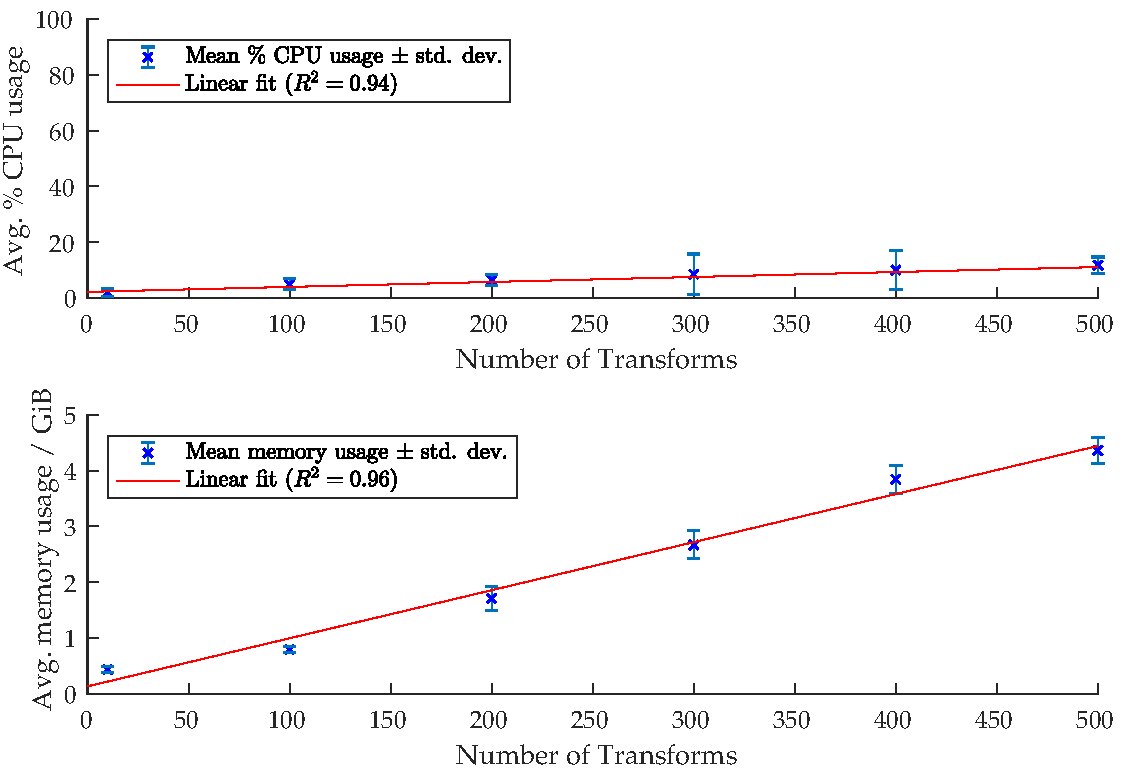
\includegraphics[height=0.42\textheight]{images/graphs/java_flink_memcpu_linear}
		\label{fig:eval:latency-graph-flink:cpumem}
	}
	\caption[Results of the latency experiment run executed on the Flink runner.]{The Flink runner handles the element stream at full throughput even for longer Pipelines. There is no apparent effect of Pipeline length on element latency in the range tested. Resource consumption scales linearly, but memory usage growth is quite steep even though CPU usage remains low.}
	\label{fig:eval:latency-graph-flink}
\end{figure}
